%%%%%%%%%%%%%%%%%%%%%%%%%%%%%%%%%%%%%%%%%
% Journal Article
% LaTeX Template
% Version 1.3 (9/9/13)
%
% This template has been downloaded from:
% http://www.LaTeXTemplates.com
%
% Original author:
% Frits Wenneker (http://www.howtotex.com)
%
% License:
% CC BY-NC-SA 3.0 (http://creativecommons.org/licenses/by-nc-sa/3.0/)
%
%%%%%%%%%%%%%%%%%%%%%%%%%%%%%%%%%%%%%%%%%

%----------------------------------------------------------------------------------------
%	PACKAGES AND OTHER DOCUMENT CONFIGURATIONS
%----------------------------------------------------------------------------------------

\documentclass[twoside]{article}

\usepackage{graphicx} % Package to include images

\usepackage{amsmath}

\usepackage[sc]{mathpazo} % Use the Palatino font
\usepackage[T1]{fontenc} % Use 8-bit encoding that has 256 glyphs
\linespread{1.05} % Line spacing - Palatino needs more space between lines
\usepackage{microtype} % Slightly tweak font spacing for aesthetics

\usepackage{mathtools}
\DeclarePairedDelimiter\abs{\lvert}{\rvert}%

\usepackage[hmarginratio=1:1,top=32mm,columnsep=20pt]{geometry} % Document margins
\usepackage{multicol} % Used for the two-column layout of the document
\usepackage[hang, small,labelfont=bf,up,textfont=it,up]{caption} % Custom captions under/above floats in tables or figures
\usepackage{booktabs} % Horizontal rules in tables
\usepackage{float} % Required for tables and figures in the multi-column environment - they need to be placed in specific locations with the [H] (e.g. \begin{table}[H])
\usepackage[hidelinks]{hyperref} % For hyperlinks in the PDF

\usepackage{lettrine} % The lettrine is the first enlarged letter at the beginning of the text
%\usepackage{paralist} % Used for the compactitem environment which makes bullet points with less space between them

\usepackage{abstract} % Allows abstract customization
\renewcommand{\abstractnamefont}{\normalfont\bfseries} % Set the "Abstract" text to bold
\renewcommand{\abstracttextfont}{\normalfont\small} % Set the abstract itself to small italic text

\usepackage{titlesec} % Allows customization of titles
\renewcommand\thesection{\Roman{section}} % Roman numerals for the sections
\renewcommand\thesubsection{\Roman{subsection}} % Roman numerals for subsections
\titleformat{\section}[block]{\large\scshape\centering}{\thesection.}{1em}{} % Change the look of the section titles
\titleformat{\subsection}[block]{\large}{\thesubsection.}{1em}{} % Change the look of the section titles
\usepackage{listings}
\usepackage{color}

\definecolor{Blue}{rgb}{0,0,0.5}
\definecolor{Green}{rgb}{0,0.75,0.0}
\definecolor{LightGray}{rgb}{0.6,0.6,0.6}
\definecolor{DarkGray}{rgb}{0.3,0.3,0.3}
\newcommand\matlabstyle{\lstset{language=Matlab,
   keywords={function,uint8,uint16,uint32,double,break,case,catch,continue,else,elseif,end,for,global,if,otherwise,persistent,return,switch,try,while},
   basicstyle=\ttfamily\footnotesize,
   breaklines=true,
   keywordstyle=\bfseries\color{Blue},
   commentstyle=\itshape\color{LightGray},
   stringstyle=\color{Green},
   numbers=left,
   numberstyle=\tiny\color{DarkGray},
   stepnumber=1,
   numbersep=10pt,
   backgroundcolor=\color{white},
   tabsize=2,
   showspaces=false,
   showstringspaces=false,
   captionpos=b}}


%Use command \code for code snippets
\newcommand{\code}[1]{\textnormal{\texttt{#1}}}

% Matlab environment
\lstnewenvironment{matlab}[1][]
{
\matlabstyle
\lstset{#1}
}
{}

% Matlab for external files
\newcommand\matlabexternal[2][]{{
\matlabstyle
\lstinputlisting[#1]{#2}}}

% Matlab for inline
\newcommand\matlabinline[1]{{\matlabstyle\lstinline!#1!}}

\newcommand\myfigure[1]{%
\medskip\noindent\begin{minipage}{\columnwidth}
\centering%
#1%
%figure,caption, and label go here
\end{minipage}\medskip}


\usepackage{fancyhdr} % Headers and footers
\pagestyle{fancy} % All pages have headers and footers
\fancyhead{} % Blank out the default header
\fancyfoot{} % Blank out the default footer
%\fancyhead[C]{Running title $\bullet$ November 2012 $\bullet$ Vol. XXI, No. 1} % Custom header text
\fancyfoot[RO,LE]{\thepage} % Custom footer text

%----------------------------------------------------------------------------------------
%	TITLE SECTION
%----------------------------------------------------------------------------------------

\title{\vspace{-15mm}\fontsize{24pt}{10pt}\selectfont\textbf{Neural Networks II - Learning a rule}} % Article title

\author{
\large
\hspace{6mm}\textsc{Han Kruiger} \hspace{12mm} \textsc{Maarten Terpstra}\\[2mm] % Your name
\normalsize University of Groningen \\ % Your institution
\normalsize \href{mailto:j.f.kruiger@student.rug.nl}{j.f.kruiger@student.rug.nl} \hspace{5mm} \normalsize \href{mailto:m.l.terpstra@student.rug.nl}{m.l.terpstra@student.rug.nl} % Your email address
\vspace{-5mm}
}
\date{}

%----------------------------------------------------------------------------------------

\begin{document}

\maketitle % Insert title

\thispagestyle{fancy} % All pages have headers and footers

%----------------------------------------------------------------------------------------
%	ABSTRACT
%----------------------------------------------------------------------------------------

\begin{abstract}
\noindent Aside from storing data, a perceptron can also be trained to learn a new rule.
In our analysis, a teacher perceptron with arbitrary weights separates a dataset and a student perceptron is trained to mimic the rule.
To learn the rule, the Minover algorithm has been implemented.
We have also determined the generalization error which determines the probability of disagreement between student and teacher for an arbitrary dataset. 
\end{abstract}

%----------------------------------------------------------------------------------------
%	ARTICLE CONTENTS
%----------------------------------------------------------------------------------------

\begin{multicols}{2} % Two-column layout throughout the main article text
\section{Introduction}
\label{sec:intro}
%!TEX root = report.tex
The perceptron was seen in the previous assignment as the basic building block for complex neural networks. The previous implementation was only capable of storing rules. In this assignment it shall be discovered whether a perceptron is capable of learning a (linearly separable) rule from example data. 

To do this, a so called teacher perceptron has defined patterns with example data $\mathbb{D} = \left\{ \pmb{\xi}^\mu, S^\mu_{R} \right\} _{\mu=1}^{P}$
 with the output labels $S^\mu \pm 1$ defined as $S^\mu = \mbox{sign}(\mathbf{w}^{*} \cdot \pmb{\xi}^\mu)$. 

In order to learn a rule, a student perceptron must be able to derive the rule as the examples are separated by the teacher. Because the separation by the teacher may not be perfect it is convenient to find the weight vector that separates the two classes of data the best, i.e. the vector that has maximum stability. The perceptron of maximal stability maximizes the minimal distance between the hyperplane and the examples\cite{perceptron_slides2}. This achieves maximum distance between the separating classes, thus making it insensitive to noise or small variations in $\pmb{\xi}^\mu$.

One possible option to find this vector is by using the Min-Over algorithm. This algorithm determines the example with the lowest stability w.r.t. $\mathbf{w}(t)$. In other words, it finds 
\[ 
\mu(t)\mbox{ with } \kappa^{\mu(t)} = \underset{\nu}{\mbox{min}} 
\left\{
\kappa^\nu(t) = \frac{\mathbf{w}(t)\pmb{\xi}^{\nu} S^{\mu}_R}{\mbox{\big|}\mathbf{w}(t)\mbox{\big|}} 
\right\}
\].

After this example is found the weight vector is updated to move away from this example, thus increasing the stability. The rule shall be called learned by the student perceptron once the stabilities do not change anymore.

\section{Implementation}
\label{sec:implementation}
%!TEX root = report.tex

\section{Results}
\label{sec:results}
%!TEX root = report.tex
Performing the perceptron training algorithm produced several interesting results.
Perceptrons of sizes 25, 50 and 100 neurons were trained, with the parameter as described in the previous section. 
Using these parameters, the fraction of successful trainings, i.e. fractions of linearly separable datasets, has been obtained. 
In Figures~\ref{fig:25neurons}-\ref{fig:100neurons}, the observed success rates of the training of networks of sizes 25, 50, and 100, respectively, along with the expected success rate based on \cite{perceptron_slides2}.
\myfigure{
	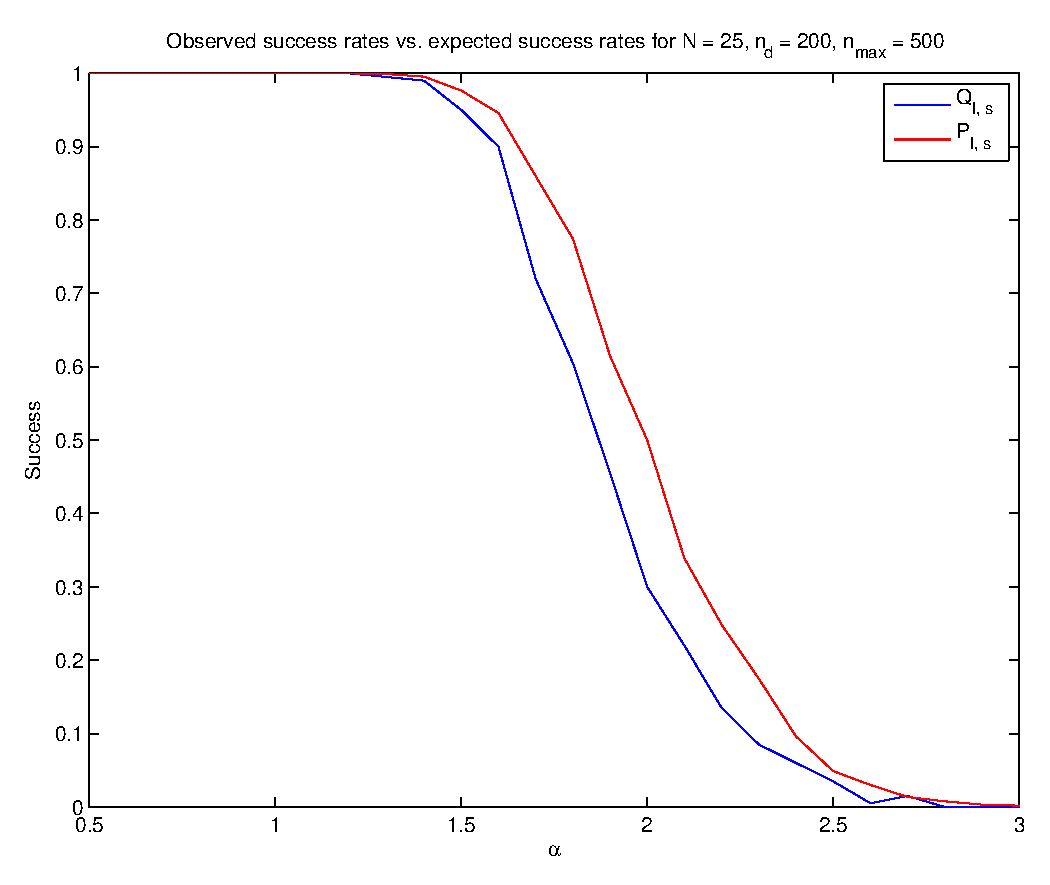
\includegraphics[width=\columnwidth]{success_rate_N_25_nd_200_nmax_500.eps}%
	\figcaption{The observed success rate (shown in blue) decreases as \(\alpha\) increases.}
	\label{fig:25neurons}
}
Figure~\ref{fig:25neurons} plots the observed success rate versus the expected success rate for 25 neurons.
It is clear that as \(\alpha\) increases the fraction of linearly separable function decreases.

\myfigure{
	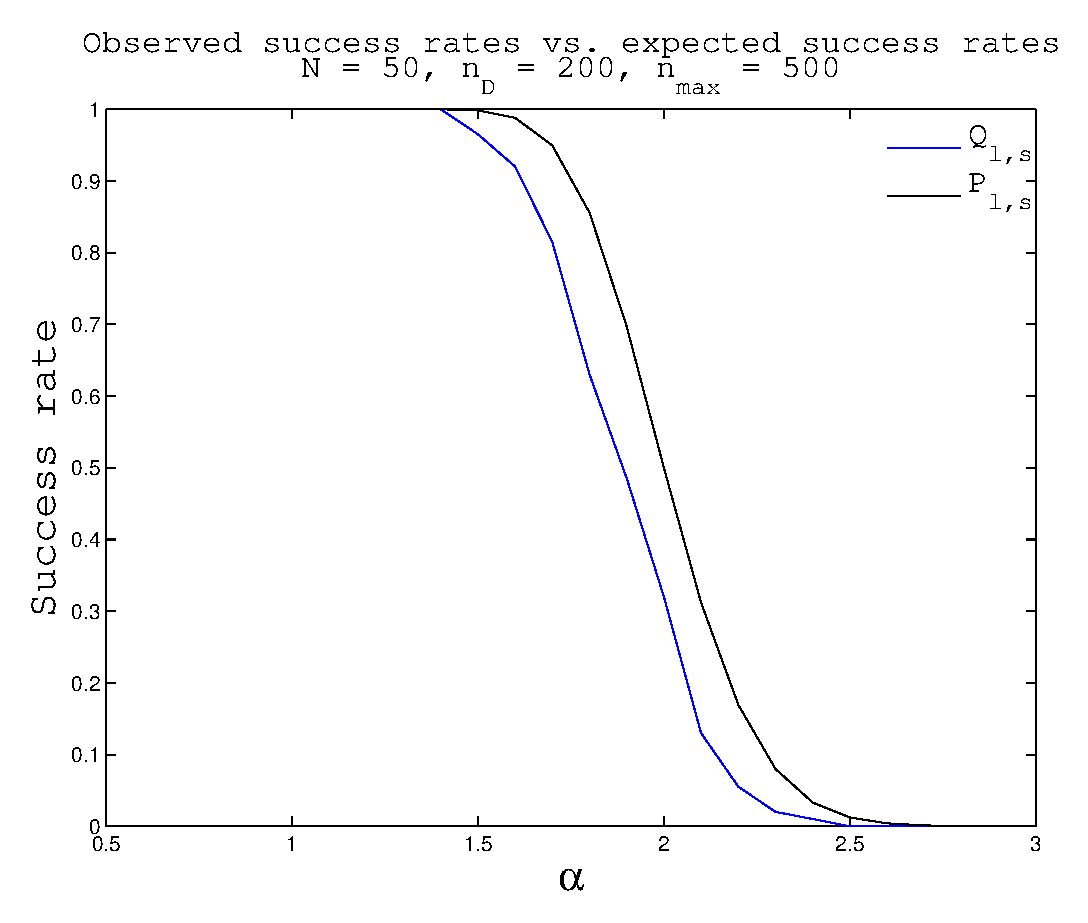
\includegraphics[width=\columnwidth]{success_rate_N_50_nd_200_nmax_500.eps}%
	\figcaption{\emph{Observed success rate versus expected success rate for 50 neurons}}
	\label{fig:50neurons}
}
Using 50 neurons as opposed to 25 neurons yields an interesting observation:
The success rate descends faster, in a smaller interval in \(\alpha\).

\myfigure{
	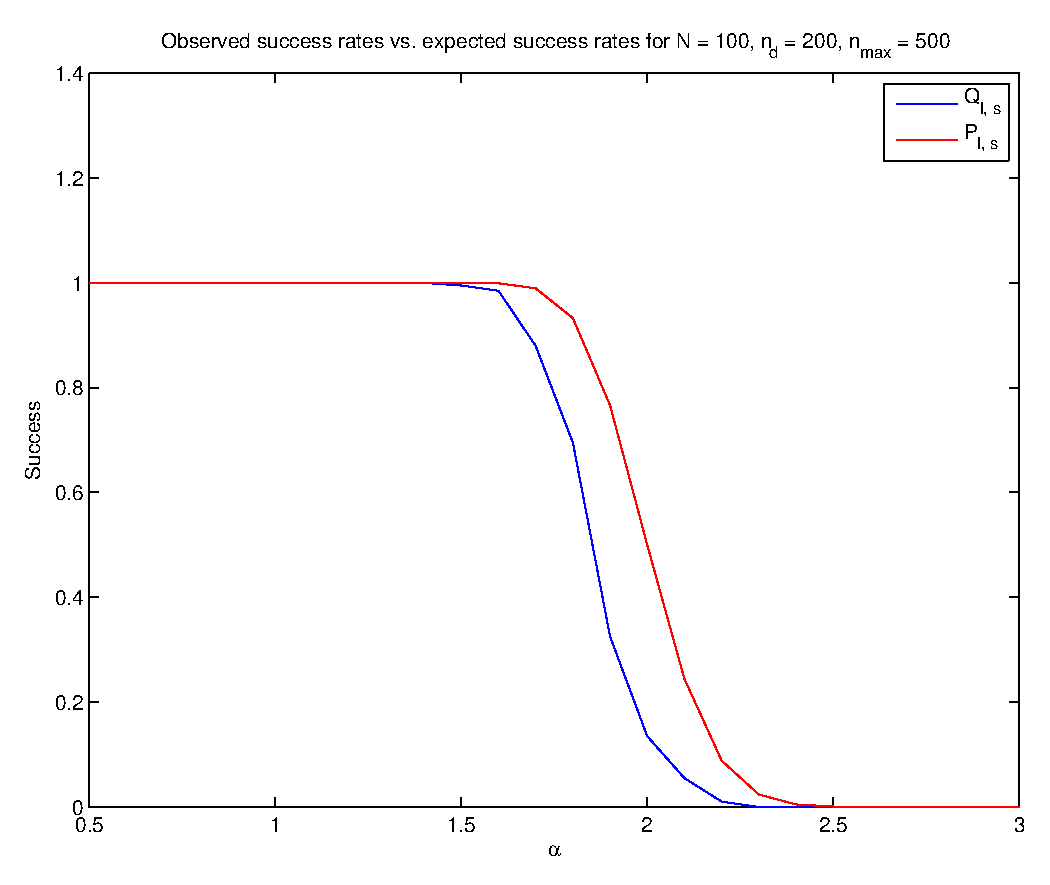
\includegraphics[width=\columnwidth]{success_rate_N_100_nd_200_nmax_500.eps}%
	\figcaption{\emph{Observed success rate versus expected success rate for 100 neurons}}
	\label{fig:100neurons}
}

When 100 neurons are used, the success rate descends even faster, and starts to resemble the step function.

\section{Discussion}
\label{sec:discussion}
%!TEX root = report.tex
One of the dangers of virtually every learning algorithm is overfitting. 
In this case, the trained model is too specific for the data and cannot correctly predict previously unforeseen observations because the generalization error increases as a result to a better fit to the training data. 
When the model is overfitted, it is highly unbiased towards the given data because it views all data as 'typical'.
As a result, the variance beyond the dataset is very large; the small fluctuations in the dataset are given too much meaning, causing it to incorrectly label data outside the trainingset.

One way to prevent overfitting is to perform the action of early stopping. 
This is a form of regularization to prevent overfitting. 
When early stopping is applied the number of iterations of algorithms as gradient descent is limited when it is detected that the machine is overfitting. 

Unfortunately, there are no formal methods to determine when to stop, as there are only ad-hoc manners to prevent overfitting. 
In our cases, we observe that overfitting can occur as soon as after 500 iterations (see figure~\ref{fig:overfitting}). 
Therefore, one way to perform early stopping for our dataset is to monitor the generalization error after 500 iterations.
If it increases as opposed to the previous iteration, the algorithm could decide to stop further training as it is starting to overfit.

\section{Conclusion}
\label{sec:conclusion}
%!TEX root = report.tex
In order to successfully implement gradient descent as a learning algorithm, one has to be careful in tuning its parameters. 
If the parameters are chosen incorrectly, the algorithm can quickly overfit (high variance) or underfit (high bias).
For our given dataset we have found that these parameters are most suited:
\begin{align*}
\eta &= 0.01 \\
P &= 500 \\
t_{max} &= 400
\end{align*}

We have found that these parameters do indeed work correctly, as Figure~\ref{fig:costs_P500} illustrates. 
The training error approaches a low value quite quickly and the test error approaches a constant value which is reasonably small (\(< 0.005\)).
We are quite pleased with these results.

\section{Workload division}
\label{sec:workload}
%!TEX root = report.tex
Here is table which describes our workload on this assignment per section. The overall percentage is how we feel we contributed individually to the entire assignment:

\begin{tabular}{ l | c | r }
    & Maarten & Han \\ \hline
  Programming & 50\% & 50\% \\
  \hline
  Introduction & 50\% & 50\% \\
  Implementation & 70\% & 30\% \\
  Results & 70\% & 30\% \\
  Discussion & 0\% & 100\% \\
  Conclusion & 60\% & 40\% \\
  \hline
  Report overall & 50\% & 50\% \\ \hline \hline
  Overall & 50\% & 50\%
\end{tabular}

%----------------------------------------------------------------------------------------
%	REFERENCE LIST
%----------------------------------------------------------------------------------------
\bibliographystyle{ieeetr}
\bibliography{sources}

%----------------------------------------------------------------------------------------

\end{multicols}
\clearpage
\appendix
\section{Code}
\matlabexternal{../minover.m}

\end{document}
